%%%%%%%%%%%%%%%%%%%%%%%%%%%%%%%%%%%%%%%%%
% Jacobs Landscape Poster
% LaTeX Template
% Version 1.1 (14/06/14)
%
% Created by:
% Computational Physics and Biophysics Group, Jacobs University
% https://teamwork.jacobs-university.de:8443/confluence/display/CoPandBiG/LaTeX+Poster
% 
% Further modified by:
% Nathaniel Johnston (nathaniel@njohnston.ca)
%
% This template has been downloaded from:
% http://www.LaTeXTemplates.com
%
% License:
% CC BY-NC-SA 3.0 (http://creativecommons.org/licenses/by-nc-sa/3.0/)
%
%%%%%%%%%%%%%%%%%%%%%%%%%%%%%%%%%%%%%%%%%

%----------------------------------------------------------------------------------------
%	PACKAGES AND OTHER DOCUMENT CONFIGURATIONS
%----------------------------------------------------------------------------------------

\documentclass[final]{beamer}

\usepackage[scale=1.24]{beamerposter} % Use the beamerposter package for laying out the poster

\usetheme{confposter} % Use the confposter theme supplied with this template

\setbeamercolor{block title}{fg=ngreen,bg=white} % Colors of the block titles
\setbeamercolor{block body}{fg=black,bg=white} % Colors of the body of blocks
\setbeamercolor{block alerted title}{fg=white,bg=dblue!70} % Colors of the highlighted block titles
\setbeamercolor{block alerted body}{fg=black,bg=dblue!10} % Colors of the body of highlighted blocks
% Many more colors are available for use in beamerthemeconfposter.sty

%-----------------------------------------------------------
% Define the column widths and overall poster size
% To set effective sepwid, onecolwid and twocolwid values, first choose how many columns you want and how much separation you want between columns
% In this template, the separation width chosen is 0.024 of the paper width and a 4-column layout
% onecolwid should therefore be (1-(# of columns+1)*sepwid)/# of columns e.g. (1-(4+1)*0.024)/4 = 0.22
% Set twocolwid to be (2*onecolwid)+sepwid = 0.464
% Set threecolwid to be (3*onecolwid)+2*sepwid = 0.708

\newlength{\sepwid}
\newlength{\onecolwid}
\newlength{\twocolwid}
\newlength{\threecolwid}
\setlength{\paperwidth}{48in} % A0 width: 46.8in
\setlength{\paperheight}{36in} % A0 height: 33.1in
\setlength{\sepwid}{0.024\paperwidth} % Separation width (white space) between columns
\setlength{\onecolwid}{0.22\paperwidth} % Width of one column
\setlength{\twocolwid}{0.464\paperwidth} % Width of two columns
\setlength{\threecolwid}{0.708\paperwidth} % Width of three columns
\setlength{\topmargin}{-0.5in} % Reduce the top margin size
%-----------------------------------------------------------

\usepackage{graphicx}  % Required for including images
\usepackage{hyperref}
\usepackage{natbib}

\usepackage{booktabs} % Top and bottom rules for tables
\usepackage{microtype}
\usepackage[linesnumbered,vlined,ruled]{algorithm2e} % algorithm

%----------------------------------------------------------------------------------------
%	TITLE SECTION 
%----------------------------------------------------------------------------------------

\title{The Parareal Algorithm for Parallel Solution of ODEs} % Poster title

\author{Wesley Chen, Brandon Sim, Andy Shi} % Author(s)

\institute{Harvard University, Applied Math 205 Final Project} % Institution(s)

%----------------------------------------------------------------------------------------

\begin{document}

\addtobeamertemplate{block end}{}{\vspace*{2ex}} % White space under blocks
\addtobeamertemplate{block alerted end}{}{\vspace*{2ex}} % White space under highlighted (alert) blocks

\setlength{\belowcaptionskip}{2ex} % White space under figures
\setlength\belowdisplayshortskip{2ex} % White space under equations

\begin{frame}[t] % The whole poster is enclosed in one beamer frame

\begin{columns}[t] % The whole poster consists of three major columns, the second of which is split into two columns twice - the [t] option aligns each column's content to the top

\begin{column}{\sepwid}\end{column} % Empty spacer column

\begin{column}{\onecolwid} % The first column

%----------------------------------------------------------------------------------------
%	OBJECTIVES
%----------------------------------------------------------------------------------------

\begin{alertblock}{Abstract}

We implement the Parareal algorithm to solve various ODEs and compare in
terms of accuracy, speedup and efficiency. We explore the effect of using
different solution operators (a coarse and a fine as required by the method).
Our code is written in python using mpi4py to parallelize. We observe
light speedups in our small scale tests up to 64 processors on Harvard's
Odyssey cluster. We analyze possible reasons as to why our implementation
may not be ideal and some tradeoffs that are taken in the Parareal
implementation. Further optimizations are proposed and rationalized as next
steps including ports of to C++ and BLAS libraries which is a more
performance-oriented, lower-level language than Python. Data is shown for
solving for various complexities of ODEs from the basic exponential to
modeling sound wave propagation as we did in homework 4.

\end{alertblock}

%----------------------------------------------------------------------------------------
%	INTRODUCTION
%----------------------------------------------------------------------------------------

\begin{block}{Algorithm}

The Parareal algorithm, developed by Lions, Maday and Turinici in 2001, is
a general algorithm that allows parallelization in time.sIt does so by using a
cheaper (lower order, lesser resolution) approximation first, and then makes
corrections in parallel. The entire process is then iterative and tuned for a
given amount of iterations. Therefore, the algorithm is $k$ repetitions of a
serial coarse method updated by a finer method run in parallel for subsections.

Subscript: time index. Superscript: iteration index.

\begin{itemize}
    \item \textbf{Input}: Temporal discretization $t_n = t_0 + n \Delta t, \, n =
        1,2,\ldots,N$
    \item \textbf{Input}: Coarse scheme $g_{\Delta t}$
    \item \textbf{Input}: Finer scheme $g_{\textnormal{fine}}$
\end{itemize}

\begin{enumerate}
    \item Compute $u^1_{n+1} = g_{\Delta t}(t_n, u^1_n)$
    \item Compute the corrections $\delta g_n(u^1_n) =
        g_{\textnormal{fine}}(t_n, u^1_n) - g_{\Delta t}(t_n, u^1_n)$ in parallel
    \item Add the prediction and correction terms as $u^2_{n+1} = g_{\Delta
        t}(t_n, u^2_n) + \delta g_n(u^1_n)$
    \item Repeat steps 2 and 3, incrementing the iteration label and using
        $u^{k+1}_0 = u^1_0$ as the initial condition
\end{enumerate}
\end{block}


%----------------------------------------------------------------------------------------

\end{column} % End of the first column

\begin{column}{\sepwid}\end{column} % Empty spacer column

\begin{column}{\onecolwid} % Begin a column which is two columns wide (column 2)

%\begin{columns}[t,totalwidth=\twocolwid] % Split up the two columns wide column

%\begin{column}{\onecolwid}\vspace{-.6in} % The first column within column 2 (column 2.1)

%----------------------------------------------------------------------------------------
%	MATERIALS
%----------------------------------------------------------------------------------------


%----------------------------------------------------------------------------------------

%\end{column} % End of column 2.1

%\begin{column}{\onecolwid}\vspace{-.6in} % The second column within column 2 (column 2.2)


%----------------------------------------------------------------------------------------

%\end{column} % End of column 2.2

%\end{columns} % End of the split of column 2 - any content after this will now take up 2 columns width

%----------------------------------------------------------------------------------------
%	IMPORTANT RESULT
%----------------------------------------------------------------------------------------

% \begin{alertblock}{Important Result}

% Lorem ipsum dolor \textbf{sit amet}, consectetur adipiscing elit. Sed commodo molestie porta. Sed ultrices scelerisque sapien ac commodo. Donec ut volutpat elit.

% \end{alertblock} 

%----------------------------------------------------------------------------------------

%\begin{columns}[t,totalwidth=\twocolwid] % Split up the two columns wide column again

%\begin{column}{\onecolwid} % The first column within column 2 (column 2.1)

%----------------------------------------------------------------------------------------
%	MATHEMATICAL SECTION
%----------------------------------------------------------------------------------------

\begin{block}{Theoretical Results}

\textbf{Convergence}

Assume the coarse operator $g_{\Delta t}$ is order $m$ and is Lipshitz, and the
fine solution operator $g_{\textnormal{fine}}$ is a sufficiently accurate
approximation to the analytic operator so we may replace $g_{\textnormal{fine}}
\to g$. 

\emph{Theorem}: The order of accuracy of the Parareal method with coarse
solution operator $g_{\Delta t}$ and fine operator $g$ is $mk$. Can be proved by
induction. 

\textbf{Stability}

With the Parareal method, it is possible to combine ODE solvers. Stability
region depends on both $g_{\Delta t}$ and $g_{\textnormal{fine}}$, and the
equation being solved. 

\textbf{Runtime and Speedup}

Let's say the coarse operator runs in time $t$, and the fine operator runs in
time $Q \cdot t$. Assume we have $N$ processors and we perform $k$ correction
steps. Then, the runtime of Parareal is, assuming negligible setup and
aggregation time,

\begin{equation}
t + k(t + \frac{Qt}{N}).
\end{equation}

In order for there to be a speedup relative to the fine operator, we require
that $t + k(t + Qt/N) < Qt$, or $k < \frac{Q - 1}{1 + Q/N}$ or $N > \frac{Qk}{Q
- 1 - k}$. 

\end{block}

\begin{block}{Methods}

We implemented the Parareal algorithm in Python, using mpi4py to parallelize it.
Our coarse operator was forward Euler step, with 100 steps, while the fine
operator was forward Euler, with $Q * 100$ steps, where $Q$ is the quality
factor. We tested the Parareal algorithm on two sets of differential equations:

\[
y'(t) = f(t, y) = \lambda y, \, y(0) = 1
\]
\[
y''(t) + 2y'(t) + 5y(t) = 0, \, y(0) = 1 \, y'(0) = 0.
\]

We ran the algorithm on different numbers of processors and varied $k$ and $Q$. 

\end{block}


%----------------------------------------------------------------------------------------

\end{column} % End of column 2.1

\begin{column}{\sepwid}\end{column}

\begin{column}{\onecolwid} % The second column within column 2 (column 2.2)

%----------------------------------------------------------------------------------------
%	METHODS
%----------------------------------------------------------------------------------------

%----------------------------------------------------------------------------------------
%	RESULTS
%----------------------------------------------------------------------------------------

\begin{block}{Preliminary Results}

\begin{figure}
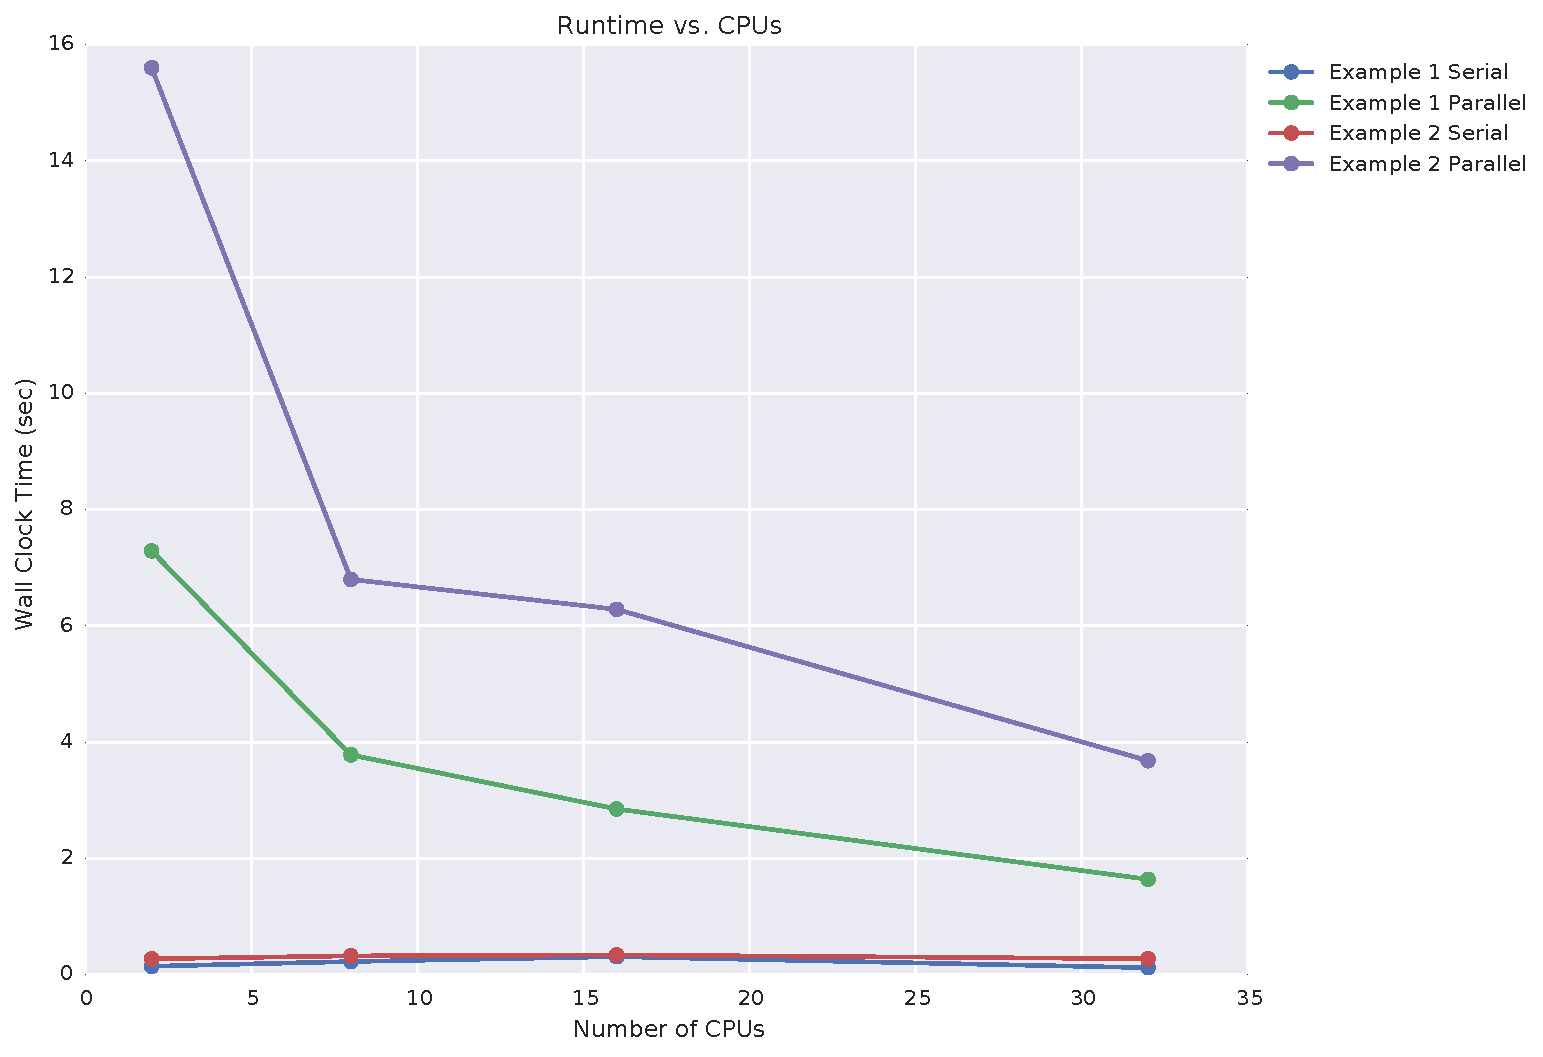
\includegraphics[width=0.75\textwidth]{../data/runtime_vs_cpus.pdf}
\caption{Running time vs. number of CPUs.}
\label{fig:run_v_cpu}
\end{figure}

\begin{figure}
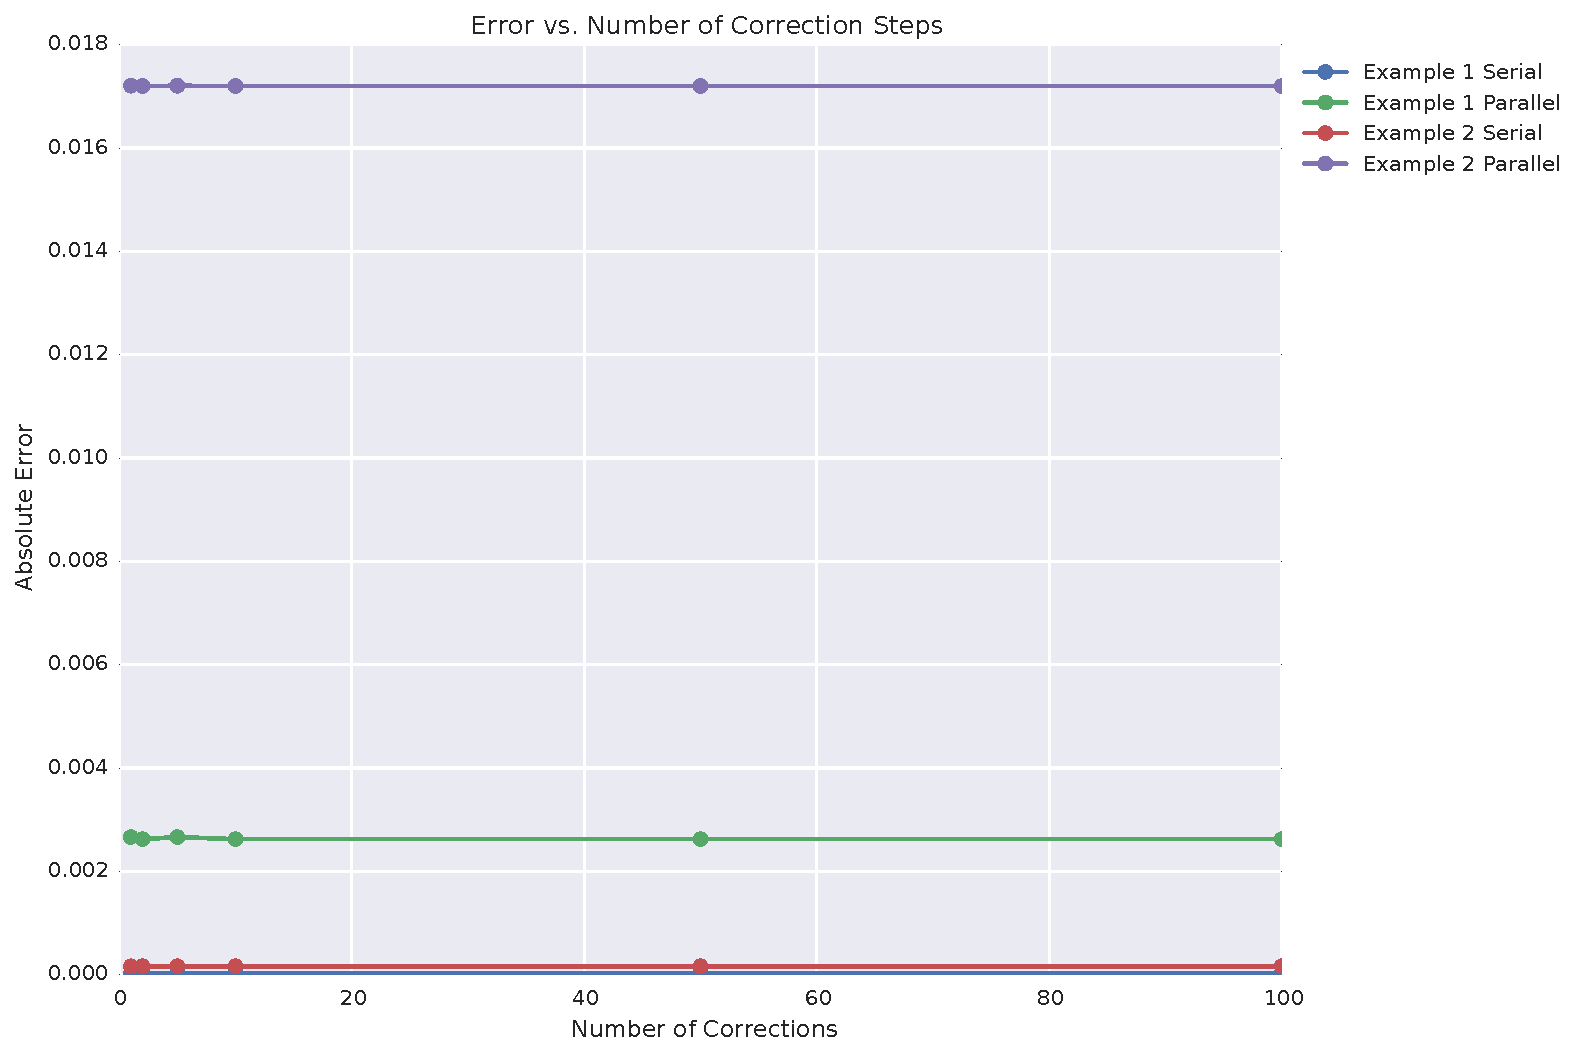
\includegraphics[width=0.75\linewidth]{../data/error_vs_corrections.pdf}
\caption{Error vs. number of correction steps.}
\label{fig:err_v_k}
\end{figure}

\begin{figure}
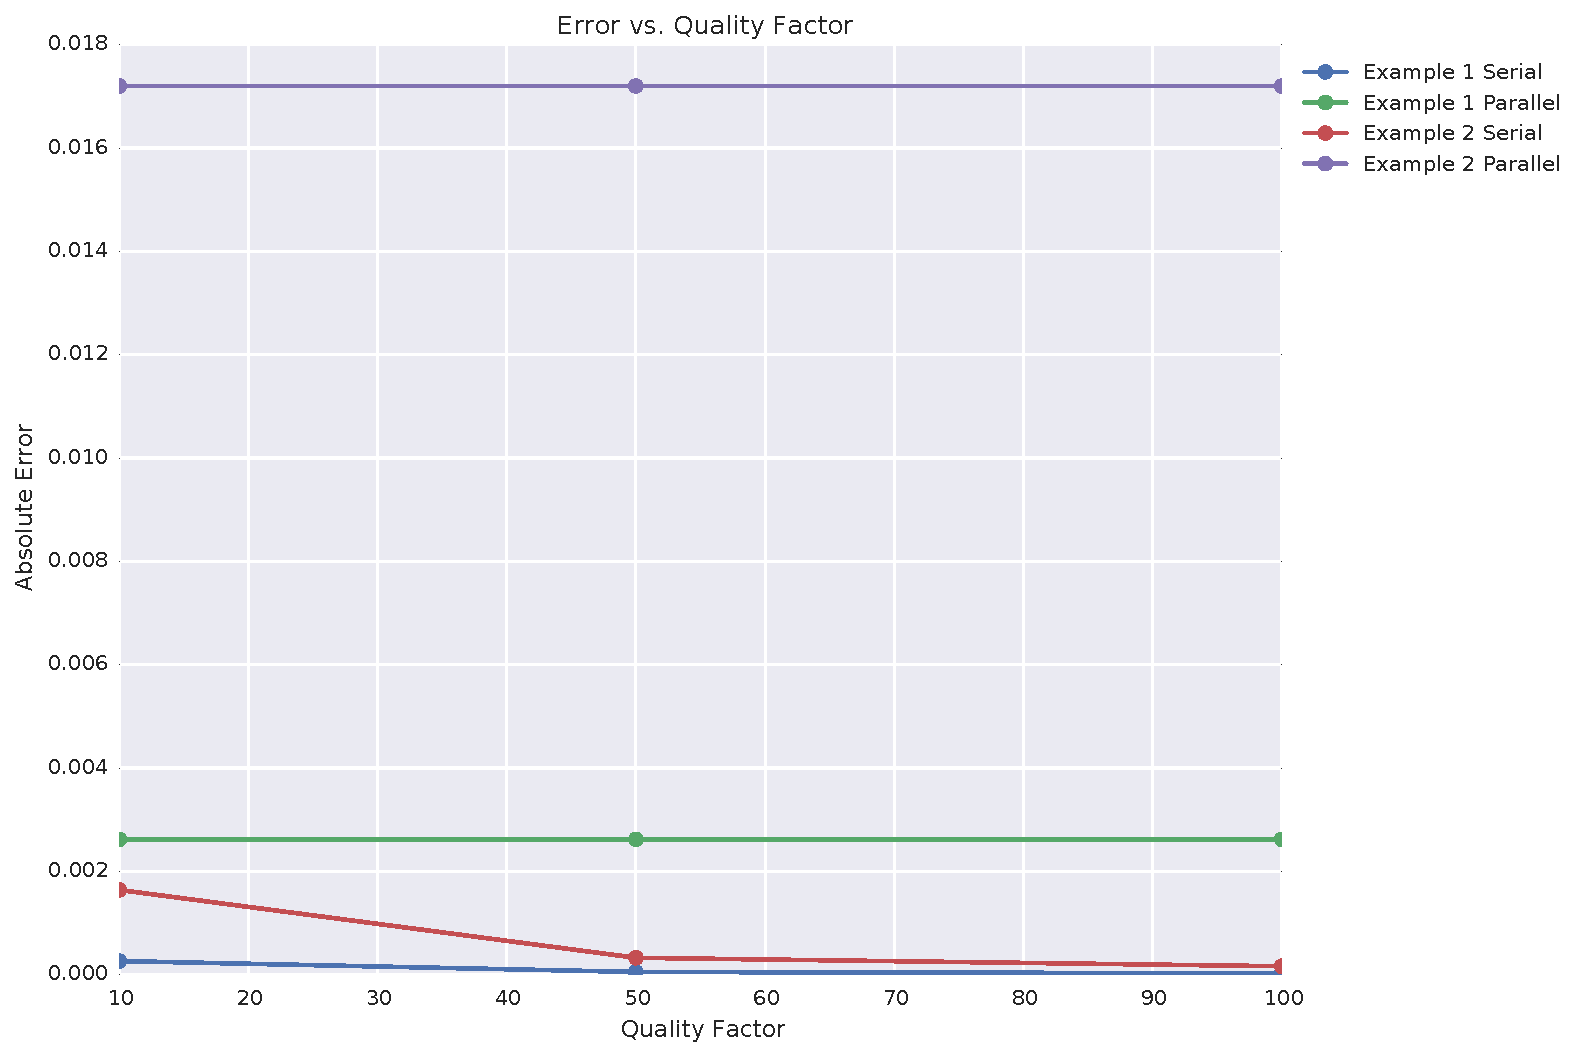
\includegraphics[width=0.75\linewidth]{../data/error_vs_qualityfactor.pdf}
\caption{Error vs. quality factor of the fine operator}
\label{fig:err_v_q}
\end{figure}

\begin{figure}
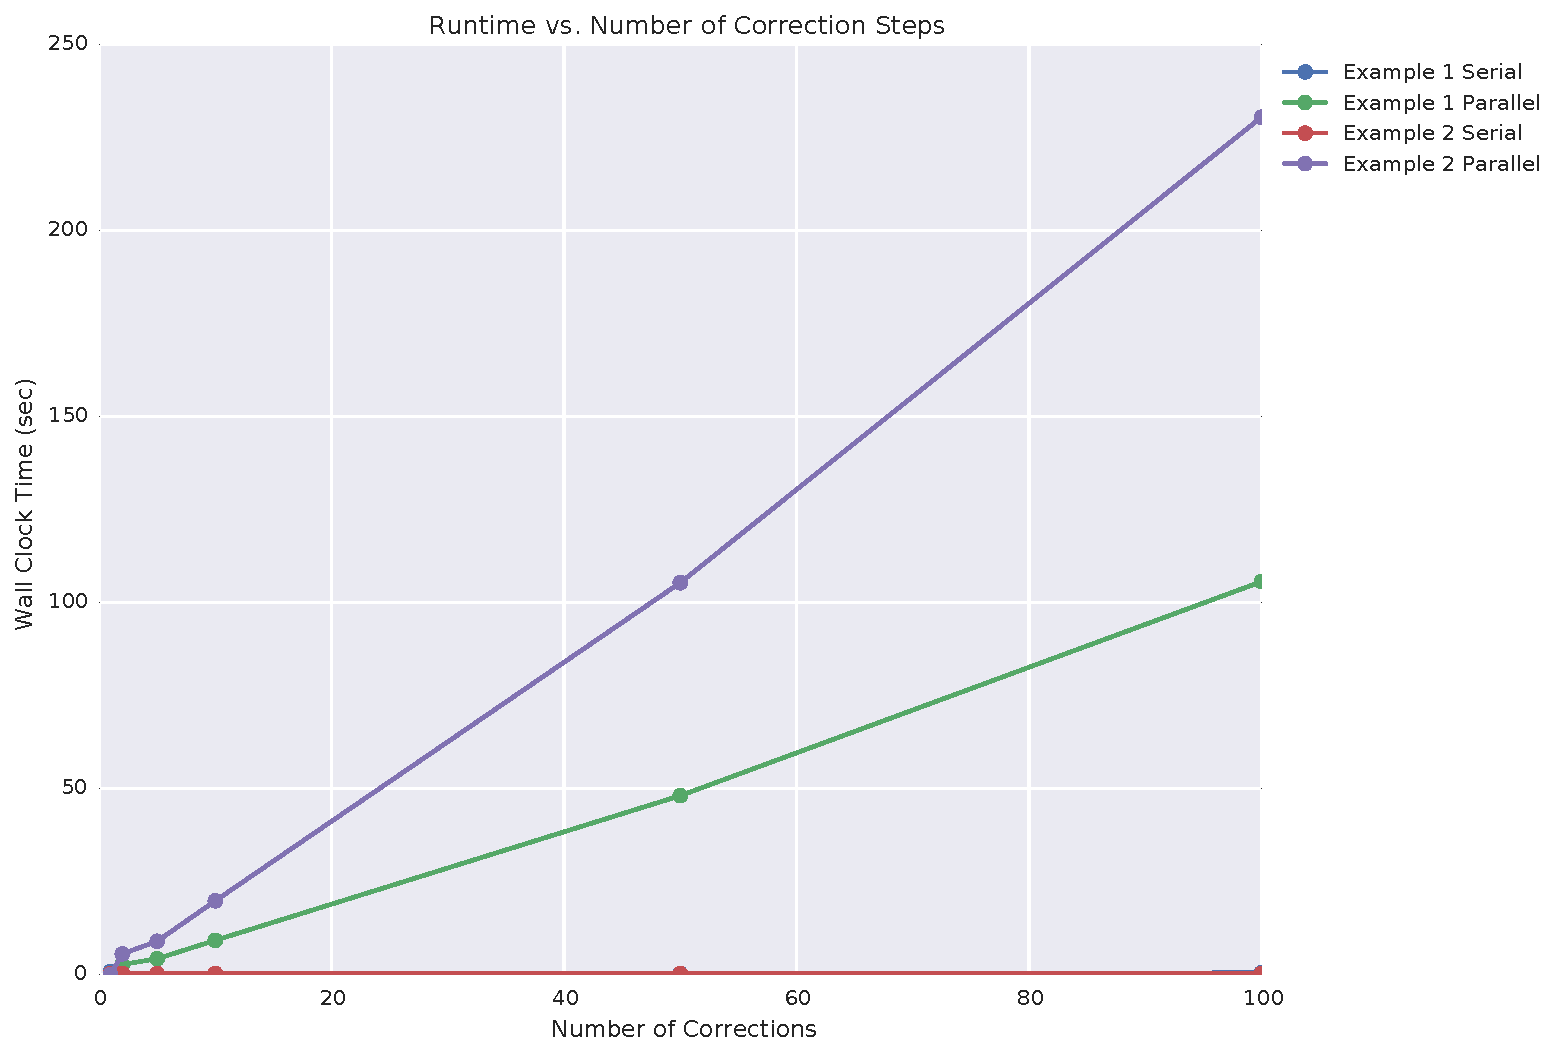
\includegraphics[width=0.75\linewidth]{../data/runtime_vs_corrections.pdf}
\caption{Running time as a function of the number of correction steps.}
\label{fig:run_v_k}
\end{figure}

\end{block}

%----------------------------------------------------------------------------------------

\end{column} % End of column 2.2

%\end{columns} % End of the split of column 2

%\end{column} % End of the second column

\begin{column}{\sepwid}\end{column} % Empty spacer column

\begin{column}{\onecolwid} % The third column

%----------------------------------------------------------------------------------------
%	CONCLUSION
%----------------------------------------------------------------------------------------

\begin{block}{Conclusion}

\end{block}

%----------------------------------------------------------------------------------------
%	ADDITIONAL INFORMATION
%----------------------------------------------------------------------------------------

\begin{block}{Additional Information}


\end{block}

%----------------------------------------------------------------------------------------
%	REFERENCES
%----------------------------------------------------------------------------------------

\begin{block}{References}

\nocite{*} % Insert publications even if they are not cited in the poster
\small{\bibliographystyle{unsrt}
\bibliography{sample}\vspace{0.75in}}

\end{block}

%----------------------------------------------------------------------------------------
%	ACKNOWLEDGEMENTS
%----------------------------------------------------------------------------------------

\setbeamercolor{block title}{fg=red,bg=white} % Change the block title color

\begin{block}{Acknowledgements}

\small{\rmfamily{Nam mollis tristique neque eu luctus. Suspendisse rutrum congue nisi sed convallis. Aenean id neque dolor. Pellentesque habitant morbi tristique senectus et netus et malesuada fames ac turpis egestas.}} \\

\end{block}

%----------------------------------------------------------------------------------------
%	CONTACT INFORMATION
%----------------------------------------------------------------------------------------

\setbeamercolor{block alerted title}{fg=black,bg=norange} % Change the alert block title colors
\setbeamercolor{block alerted body}{fg=black,bg=white} % Change the alert block body colors

\begin{alertblock}{Contact Information}

\begin{itemize}
\item Web: \href{http://www.university.edu/smithlab}{http://www.university.edu/smithlab}
\item Email: \href{mailto:john@smith.com}{john@smith.com}
\item Phone: +1 (000) 111 1111
\end{itemize}

\end{alertblock}

\begin{center}

\includegraphics[width=0.2\linewidth]{seas-rgb.png}
\end{center}

%----------------------------------------------------------------------------------------

\end{column} % End of the third column

\end{columns} % End of all the columns in the poster

\end{frame} % End of the enclosing frame

\end{document}
